\documentclass{standalone}

% Preamble
\begin{document}

  \subsection{Calcul numérique des racines}
  Nous reprenons l'exemple ci-dessus. La matrice de Bezout $B(1)$, à coefficients entiers, est de taille \input{../txt/Dx.txt}. Après réductions on trouve que la dimension du quotient $A$ est \input{../txt/dim.txt}. En calculant numériquement les valeurs propres des matrices compagnon $X_j = B(x_j)B(1)^{-1}$ on obtient les racines du système polynômial $f$. On vérifie la qualité de chacune des racines obtenues en lui appliquant les polynômes $f_i, i=1,\cdots,n$. Les résultats sont représentés sous forme d'histogramme o\`u le logarithme décimal de l'erreur est porté en abscisse.
\begin{figure}[!ht]
  \centering
    \caption{Processus de réduction exécuté en arithmétique exacte}
  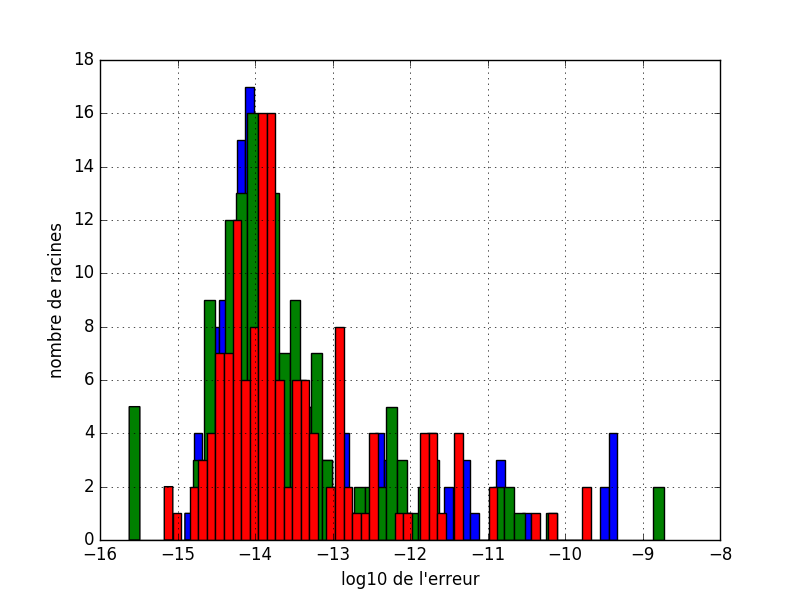
\includegraphics[height=8cm, width=0.8\textwidth]{../png/sage_roots.png}
\end{figure}
 Sur la figure suivante le processus de réduction est effectué en arithmétique flottante.
 \begin{figure}[!ht]
   \centering
     \caption{Processus de réduction exécuté en arithmétique flottante}
   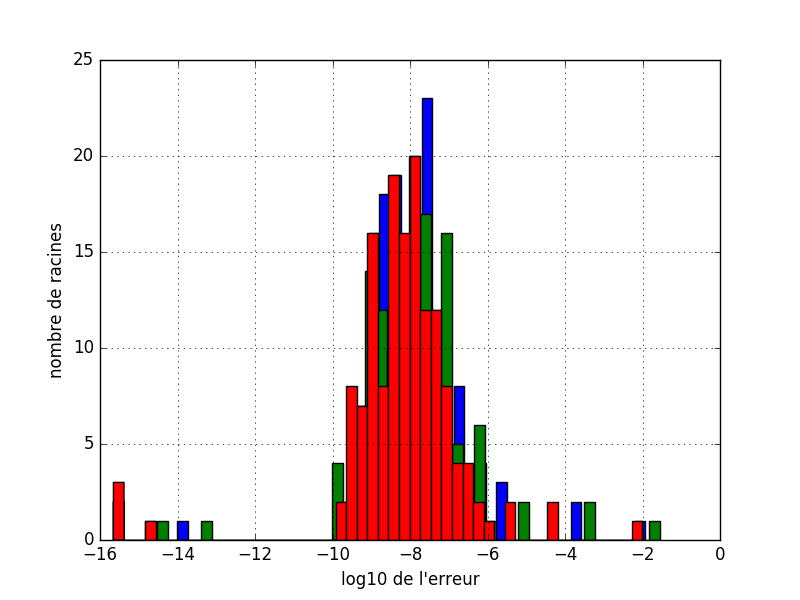
\includegraphics[height=8cm, width=0.8\textwidth]{../png/octave_roots.png}
 \end{figure}
 On constate que le temps de calcul en arithmétique flottante est plus court mais au prix d'une dégradation sensible de la qualité des résultats.
\begin{table}
    \caption{timings}
\begin{tabular}{l|llr}
  Arithmétique & Processus & Software & Timing \\ \hline
  \multirow{4}{*}{flottante} & Construction matrices de Bezout & NumPy & $\input{../txt/construction_B_time.txt}$ ms \\ %\hline
   & Noyau de $B(1)$ & Octave & $\input{../txt/octave_triang_time.txt}$ ms \\
   & Réduction matrices & Octave & $\input{../txt/octave_reduct_time.txt}$ ms \\ %\hline
   & Valeurs propres & SciPy & $\input{../txt/eigenstructure_time.txt}$ ms \\ \hline \hline
  \multirow{2}{*}{exacte} & Réduction matrices & SageMath & $\input{../txt/sage_reduct_time.txt}$ ms \\ %\hline
   & Vérification dimension Algèbre & Sage & $\input{../txt/sage_dimension_time.txt}$ ms
\end{tabular}
\end{table}



\end{document}
